\section{连通器}\label{sec:5-8}

用橡皮管把两根玻璃管连通起来。先用夹子夹住橡皮管,向一根玻璃管里灌水。
然后松开夹子,水就从这根管流向另一根管,直到两根管里的水面相平为止(图 \ref{fig:5-28})。

\begin{figure}[htbp]
    \centering
    \begin{minipage}{5cm}
    \centering
    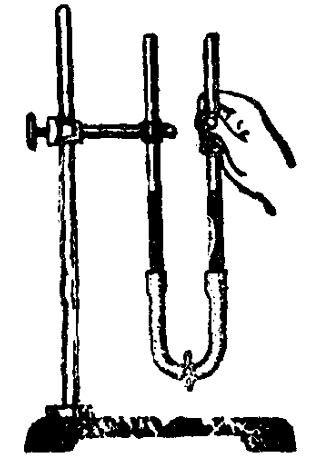
\includegraphics[width=3cm]{../pic/czwl1-ch5-28}
    \caption{}\label{fig:5-28}
    \end{minipage}
    \qquad
    \begin{minipage}{9cm}
    \centering
    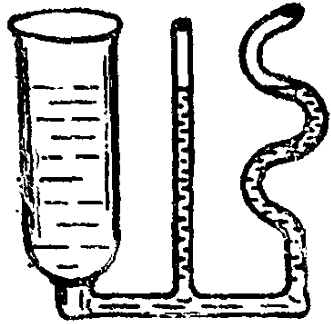
\includegraphics[width=4cm]{../pic/czwl1-ch5-29}
    \caption{}\label{fig:5-29}
    \end{minipage}
\end{figure}

把一根管固定在铁架上,使另一根管升高、下降或倾斜,可以看到两根管里的水面总保持相平。

向几个底部互相连通的容器中灌水,可以看到,在水不流动的时候,各个容器中的水面是相平的(图 \ref{fig:5-29})。

\textbf{底部互相连通的容器叫做连通器}。上面的实验表明,连通器里如果只有一种液体,
在液体不流动的情况下,各容器中的液面总保持相平。

这个现象可以用图 \ref{fig:5-30} 来解释。

设想在连通器下部正中有一个小液片 $AB$。
如果液体不流动,左边液柱对液片 $AB$ 向右的压强,一定等于右边液柱对液片 $AB$ 向左的压强。
管里装的是一种液体,左右两边液柱的密度相同,根据液体压强的公式 $p = \rho gh$,可以知道,
只有两边液柱的高度相等,两边液柱对液片 $AB$ 的压强才能相等。
所以在液体不流动的情况下,连通器各容器中的液面应保持相平。

\begin{figure}[htbp]
    \centering
    \begin{minipage}{5cm}
    \centering
    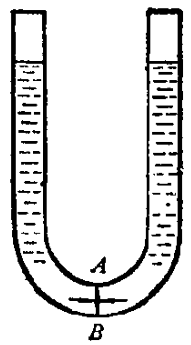
\includegraphics[width=2.5cm]{../pic/czwl1-ch5-30}
    \caption{}\label{fig:5-30}
    \end{minipage}
    \qquad
    \begin{minipage}{9cm}
    \centering
    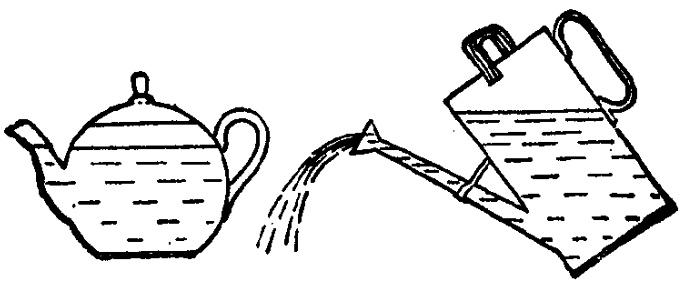
\includegraphics[width=8cm]{../pic/czwl1-ch5-31}
    \caption{}\label{fig:5-31}
    \end{minipage}
\end{figure}

连通器的道理虽然很简单,但是在生产和生活中却有广泛的应用。下面举几个例子。

日常生活中用的茶壶、酒水壶等就是连通器(图 \ref{fig:5-31})。
壶身和壶嘴互相连通, 因此壶嘴里的水面总是跟壶身里的水面相平。
当壶身倾斜时,水就从壶嘴里流出来。壶嘴总是跟壶身一样高的,想想看,
如果壶嘴比壶身低,壶身里还能装满水吗?

锅炉里的水位需要保持一定的高度,水位过低,锅炉就有爆炸的危险。
为了随时了解锅炉内的水位.在锅炉上都装有水位计。水位计和锅炉就构成一个连通器(图 \ref{fig:5-32})。

\begin{figure}[htbp]
    \centering
    \begin{minipage}{5cm}
    \centering
    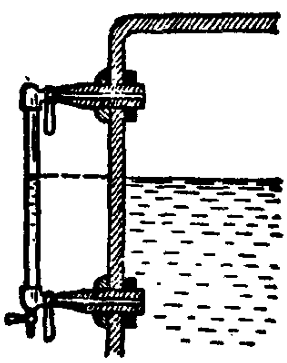
\includegraphics[width=3cm]{../pic/czwl1-ch5-32}
    \caption{锅炉水位计}\label{fig:5-32}
    \end{minipage}
    \qquad
    \begin{minipage}{9cm}
    \centering
    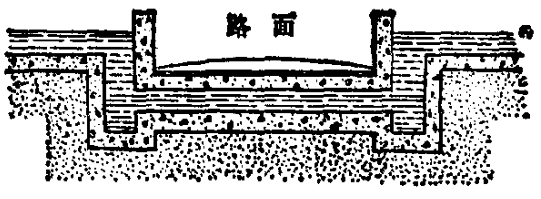
\includegraphics[width=7cm]{../pic/czwl1-ch5-33}
    \caption{过路涵洞}\label{fig:5-33}
    \end{minipage}
\end{figure}

在水渠通过公路的地方,为了不妨碍交通,要修建过路涵洞,让水从公路下面流过再翻到地面上来(图 \ref{fig:5-33})。
过路涵洞也是个连通器。

